\section{MSSQL implementation. Particularities}
\subsection{Preparing database}
\subsubsection{Downloading database}
In this Course Work I will use database Adventure Works \cite{AdventureWorks}. 
\begin{figure}[ht!]
	\centering
	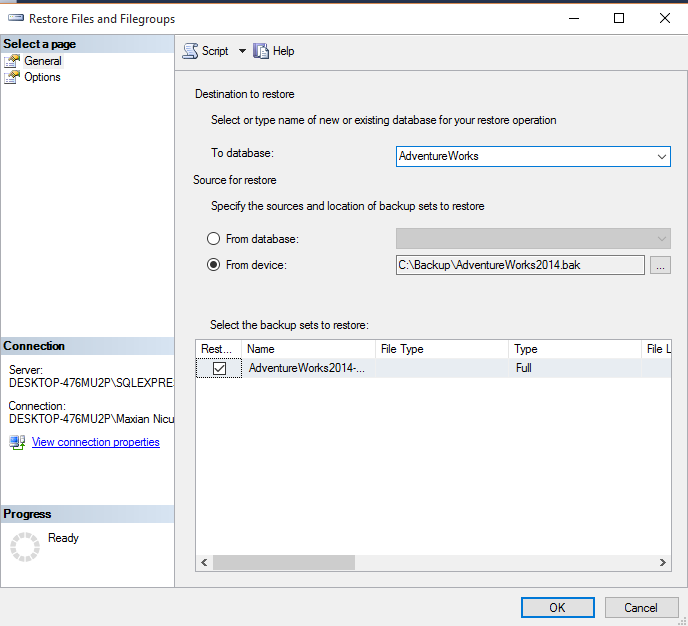
\includegraphics[width=0.8\textwidth]{restore}
	\caption{Restoring AdventureWorks database}
\end{figure}

\subsubsection{Droping database indexes}
In order to show why we should use indexes, let remove all indexes for following tables:
\begin{itemize}
	\item Production.Product
	\item Production.ProductCategory
	\item Person.EmailAddress
	\item Person.Password
	\item Person.Person
	\item Person.PersonPhone\textsl{}
	\item Person.PhoneNumberType
\end{itemize}

\subsection{Clustered Indexes}
\subsubsection{Problem definition}
Let's assume we have following query, which extracts ProductId, Name,Category and StandartCost from database.
\lstinputlisting[style=mystyle, language=SQL, caption={Finding product with a given id}]{sourcecode/productSearch.sql}

\subsubsection{Analysis of execution plan}
\begin{figure}[ht!]
	\centering
	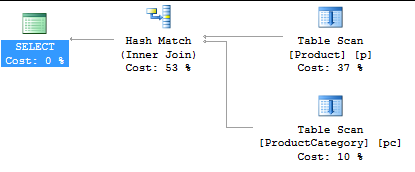
\includegraphics[width=0.5\textwidth]{product_find}
	\caption{Execution plan for the query}
\end{figure}

From this execution plan, we see that our query has cost of \textbf{0.034}. Furthermore, since our tables have no clustered indexes, data is stored as a heap, in the file. We see that our algorithm scans table for finding needed row. This means that query takes row by row and tries to find needed row that matches our criterions. This is ok for few rows, but when we have thousands of rows, performance will hurt us. 

\subsubsection{Solution}
Of course Clustered Indexes. Clustered Indexes rearranges our table data as a b-tree structure. Let's create clustered index on Product table, with column ProductId. Now we can find needed product at once, without scanning all entire data ! Once we found product, we have also ProductSubCategoryId, which is also an clustered index for ProductCategory table, so we access that table also by id.


\lstinputlisting[style=mystyle, language=SQL, caption={Creating clustered indexes}]{sourcecode/productIndexes.sql}

\subsubsection{Final results}

\begin{figure}[ht!]
	\centering
	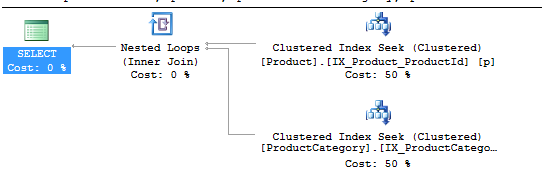
\includegraphics[width=0.6\textwidth]{product_after_indexes}
	\caption{Execution plan after creating clustered indexes}
\end{figure}

Now we can see that we have \textbf{Clustered Index Seek}. This is faster way to find a data. This means we have no more loops, scan and everything that costs us data. Having ProductID, we can directly access Address of data, where row is situated. So, we have optimized our query as much as possible ! Now we have total cost of \textbf{0.0065}, 80\% less than initial. That is awesome !



\subsection{Non Clustered Indexes}
\subsubsection{Problem definition}
Here we will try to extract basic data such as FirstName,LastName,Email,Password,PasswordHash,Phone,PhoneType for each Person based on following tables:
\begin{itemize}
	\item EmailAddress
	\item Password
	\item Person
	\item PersonPhone
	\item PhoneNumberType
\end{itemize}
\lstinputlisting[style=mystyle, language=SQL, caption={Selecting person base information}]{sourcecode/personInfo.sql}

\subsubsection{Analysis of execution plan}
\begin{figure}[ht!]
	\centering
	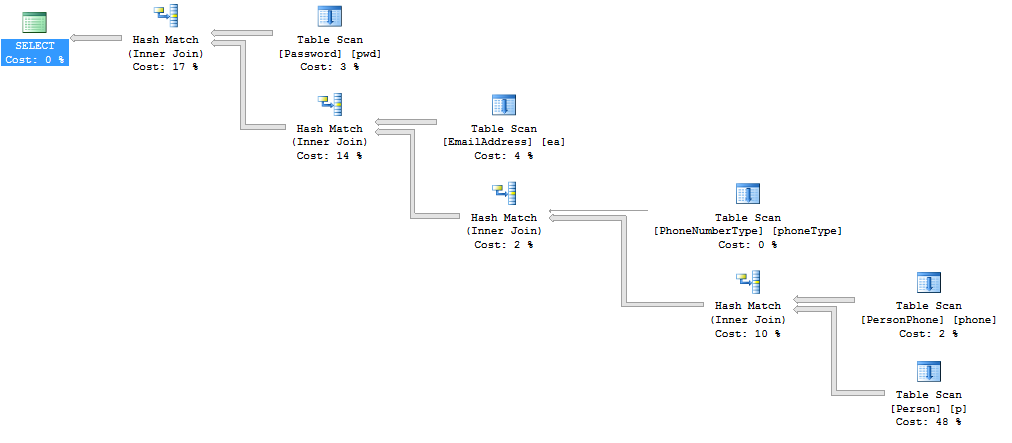
\includegraphics[width=1\textwidth]{person_analysis}
	\caption{Execution plan for the query}
\end{figure}

Hence, we obtained an cost of \textbf{5.94} for our query with 19972 rows.

Since we don't have any index here, we can observe that in execution plan we have only "Table scan". This means in our query, SQL engine scan table row by row, which is very slow. 

\subsubsection{Solution}
In order to optimize it, let's to improve our queries with Non Clustered indexes. This means that, instead of big tables we will search into smaller index tables, which contains less data and can be found with a given index.

Since we have 13 columns on \textbf{Person} table, it make us to have a big overhead when extracting data. Since we assume we will execute a lot of times this query, we need to optimize this. Non-clustered indexes are great for this. We could "shrink" our data table by creating smaller index table. We will create index on \textbf{BussinessEntittyID} column because we use this column in JOIN clauses. We also need \textbf{FirstName} and \textbf{LastName} information from that table, we also define this columns to be included into non-clustered index table. Same things we will do for each table, in order to optimize our query and remove overhead which we acutally don't need.

\lstinputlisting[style=mystyle, language=SQL, caption={Creating non-clustered indexes}]{sourcecode/personNonClusteredIndex.sql}

\subsubsection{Final results}
\begin{figure}[ht!]
	\centering
	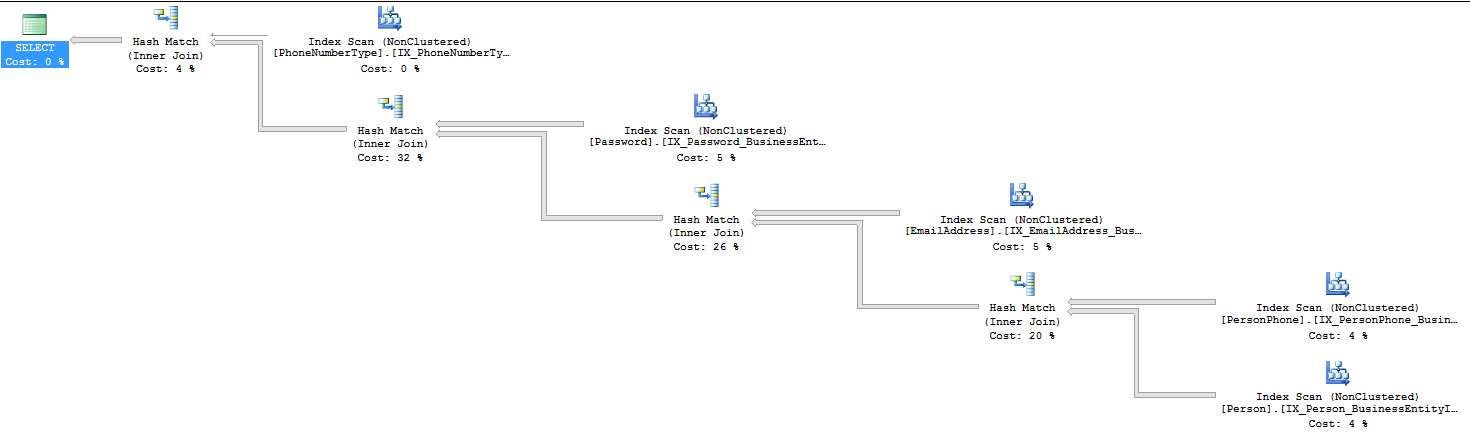
\includegraphics[width=1\textwidth]{person_analysis_after}
	\caption{Execution plan after non-clustered index creation}
\end{figure}

Now, we see that instead of table scan we have Index Scan. Which is faster than what we had. Also now we have in indexes everything what we need, so no need to lookup into the table for missing columns.

Now we have an cost of \textbf{3.12}, which is 48\% less than we had before. Nice ! It's an improvement.

\clearpage